%%%%%%%%%%%%%%%%%%%%%%%%%%%%%%%%%%%%%%%%%%%%%%%%%%%%%%%%%%%%%%%%%%%%%%%%%%%%%%%%
%2345678901234567890123456789012345678901234567890123456789012345678901234567890
%        1         2         3         4         5         6         7         8

\documentclass[letterpaper, 10 pt, conference]{ieeeconf}  % Comment this line out if you need a4paper
\usepackage{cite}
\usepackage{amsmath,amssymb,amsfonts}
\usepackage{algorithmic}
\usepackage{graphicx}
\usepackage{textcomp}
\usepackage{xcolor}

%\documentclass[a4paper, 10pt, conference]{ieeeconf}      % Use this line for a4 paper

\IEEEoverridecommandlockouts                              % This command is only needed if 
                                                          % you want to use the \thanks command

\overrideIEEEmargins                                      % Needed to meet printer requirements.

%In case you encounter the following error:
%Error 1010 The PDF file may be corrupt (unable to open PDF file) OR
%Error 1000 An error occurred while parsing a contents stream. Unable to analyze the PDF file.
%This is a known problem with pdfLaTeX conversion filter. The file cannot be opened with acrobat reader
%Please use one of the alternatives below to circumvent this error by uncommenting one or the other
%\pdfobjcompresslevel=0
%\pdfminorversion=4

% See the \addtolength command later in the file to balance the column lengths
% on the last page of the document

% The following packages can be found on http:\\www.ctan.org
%\usepackage{graphics} % for pdf, bitmapped graphics files
%\usepackage{epsfig} % for postscript graphics files
%\usepackage{mathptmx} % assumes new font selection scheme installed
%\usepackage{times} % assumes new font selection scheme installed
%\usepackage{amsmath} % assumes amsmath package installed
%\usepackage{amssymb}  % assumes amsmath package installed

\title{\LARGE \bf
Homework 2 \\
\small{UCLA MAE 263F, Fall 2024\\
Mechanics of Flexible Structures and Soft Robots}%
}


\author{He Kai Lim$^{1}$ % <-this % stops a space
\thanks{$^{1}$He Kai Lim is with the 
Department of Mechanical and Aerospace Engineering, 
University of California Los Angeles, Los Angeles, CA 90095 USA
        {\tt\small limhekai@ucla.edu}}%
}


\begin{document}

\maketitle
\thispagestyle{empty}
\pagestyle{empty}


%%%%%%%%%%%%%%%%%%%%%%%%%%%%%%%%%%%%%%%%%%%%%%%%%%%%%%%%%%%%%%%%%%%%%%%%%%%%%%%%
\begin{abstract}
   This report strives to provide all deliverables for Homework 2 in partial fulfilment of the requirements for UCLA MAE 263F, Fall 2024 (Mechanics of Flexible Structures and Soft Robots)
\end{abstract}


%%%%%%%%%%%%%%%%%%%%%%%%%%%%%%%%%%%%%%%%%%%%%%%%%%%%%%%%%%%%%%%%%%%%%%%%%%%%%%%%
\section{INTRODUCTION}

A complete simulation of three dimensional (3D) elastic rods is a fundamental building block to simulating complex structures in the real world.
This builds on prior work with 2D simulations on beams, where the fundamental physics of bending and stretching are considered.
The complexity with extension into the 3D domain stems from the inclusion of twist --- nodes can rotate about the tangential axis between each other.


%%%%%%%%%%%%%%%%%%%%%%%%%%%%%%%%%%%
\section{METHODS}

The method of discrete simulation is heavily referenced from the course notes of UCLA MAE 263F, Fall 2024.
Specific to this homework assignment, the fundamental physics incorporated in this simulation are described below.

\subsection{Elastic Energies}

We note that the total elastic energy of an elastic rod is

\begin{equation}
   E_{elastic} = \underbrace{\sum^{N-1}_{k=1}E^s_k}_{stretching} 
   + 
   \underbrace{\sum^{N-1}_{k=2}E^b_k}_{bending} 
   + 
   \underbrace{\sum^{N-1}_{k=2}E^t_k}_{twisting} 
\end{equation}

between all $N$ nodes $k$.

In the generalization from 2D to 3D, we note that $stretching$ and $bending$ energy formulations in 3D are intuitive.
The novelty in this work stems from the incorporation of \textit{twisting} energy, represented as

\begin{equation}
   \sum^{N-1}_{k=2}E^t_k = \frac{1}{2} GJ \tau^2_k \frac{1}{\bar{l}_k}
\end{equation}

where $GJ$ is the twisting stiffness (shear modulus times polar moment of inertia), $\tau_k$ is the integrated twist at node $k$.


\subsection{Simulation Scenario}

An elastic rod with a total length $l = 20 \text{cm}$ is naturally curved with radius $R_n = 2 \text{cm}$.
The location of its $N$ nodes at $t=0$ are
$$
   x_k = [R_n \cos{(k-1) \Delta \theta}, R_n \sin{(k-1) \Delta \theta}, 0]
$$
where $\Delta \theta = \frac{l}{R_n} \frac{1}{N-1}$.
The twist angles $\theta^k$ ($k=1, ..., N-1$) at $t=0$ are 0.
The first two nodes and the first twist angle remain fixed throughout the simulation (i.e. one end is clamped).
The physical parameters are: density $\rho = 1000 \text{kg}/\text{m}^3$, cross-sectional radius $r_0 = 1 \text{mm}$, Young's modulus $E = 10 \text{MPa}$ , shear modulus $G = \frac{E}{3}$ (corresponding to an incompressible material), and gravitational acceleration $g = [0, 0, -9.81]^T$.

The number of nodes $N$ and the step size $\Delta t$ are investigated in sensitivity analysis across multiple simulations thusly presented below.

%%%%%%%%%%%%%%%%%%%%%%%%%%%%%%%%%%%
\section{Results}

\subsection{General Results}

We observe that the elastic rod begins the simulation as a coiled planar circle, but stretches under gravity to become a helical coil (spring shape).
With the time available for this project, the most accurate simulation of this scenario comprised $N=400$ nodes and $\Delta t = 0.005$ s.
This simulation required 83 mins to complete computation on the author's personal computer.

% [h!] makes latex try to place figure exactly there, not floating around
\begin{figure}[h!]
   \centering
   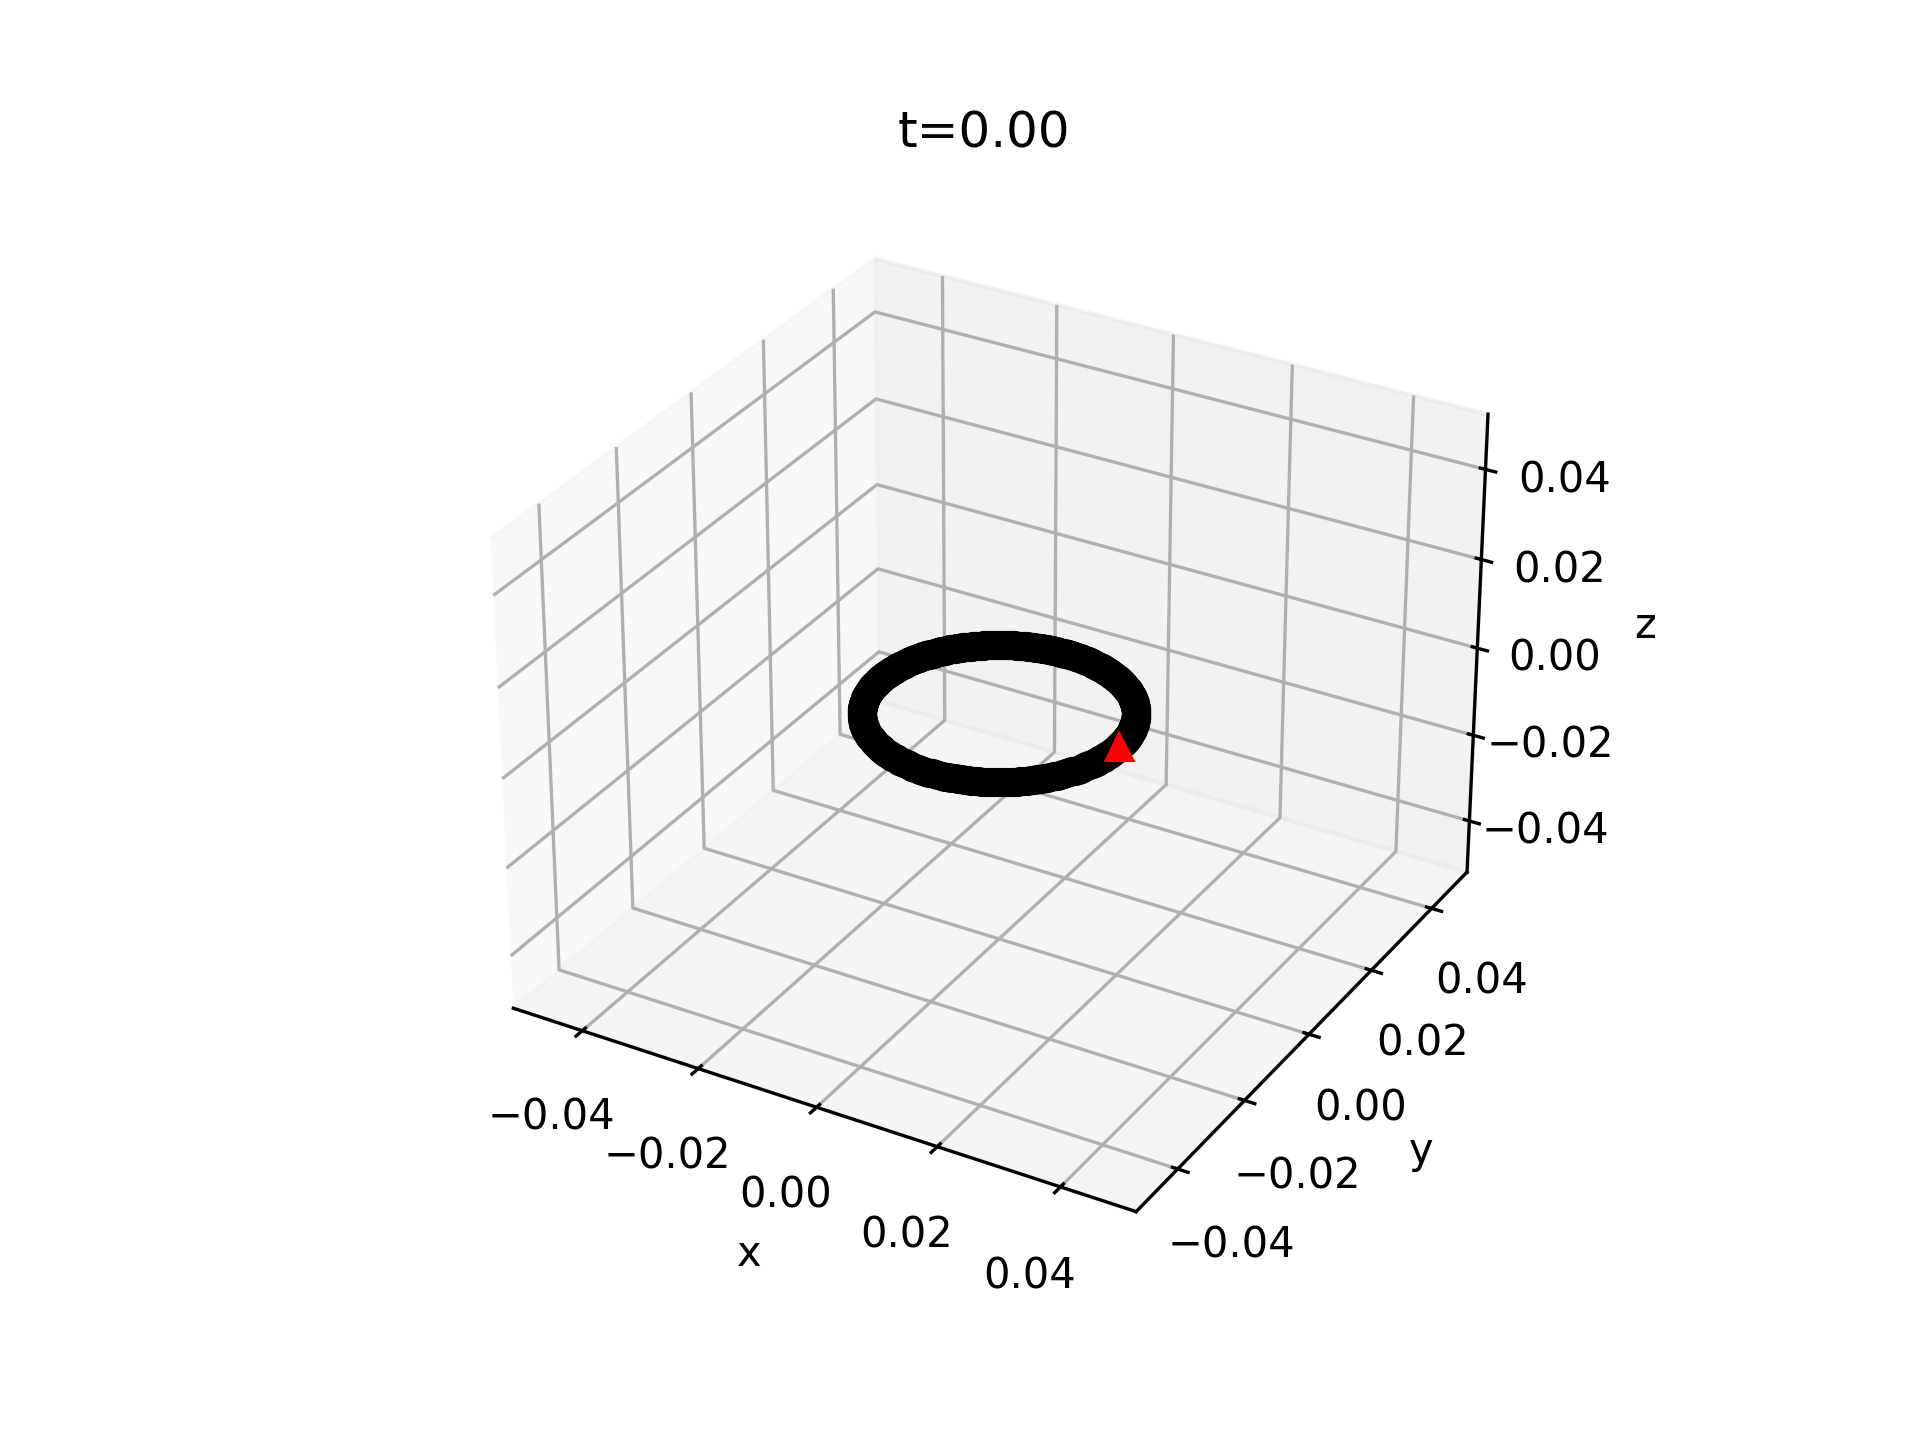
\includegraphics[width=0.8\linewidth]{../figures/n_400_dt_0-005_t=0s.png}
   \caption{The most accurate simulation, starting pose ($N=400$, $\Delta t = 0.005$s)}
   \label{fig:accurate_start}
\end{figure}

\begin{figure}[h!]
   \centering
   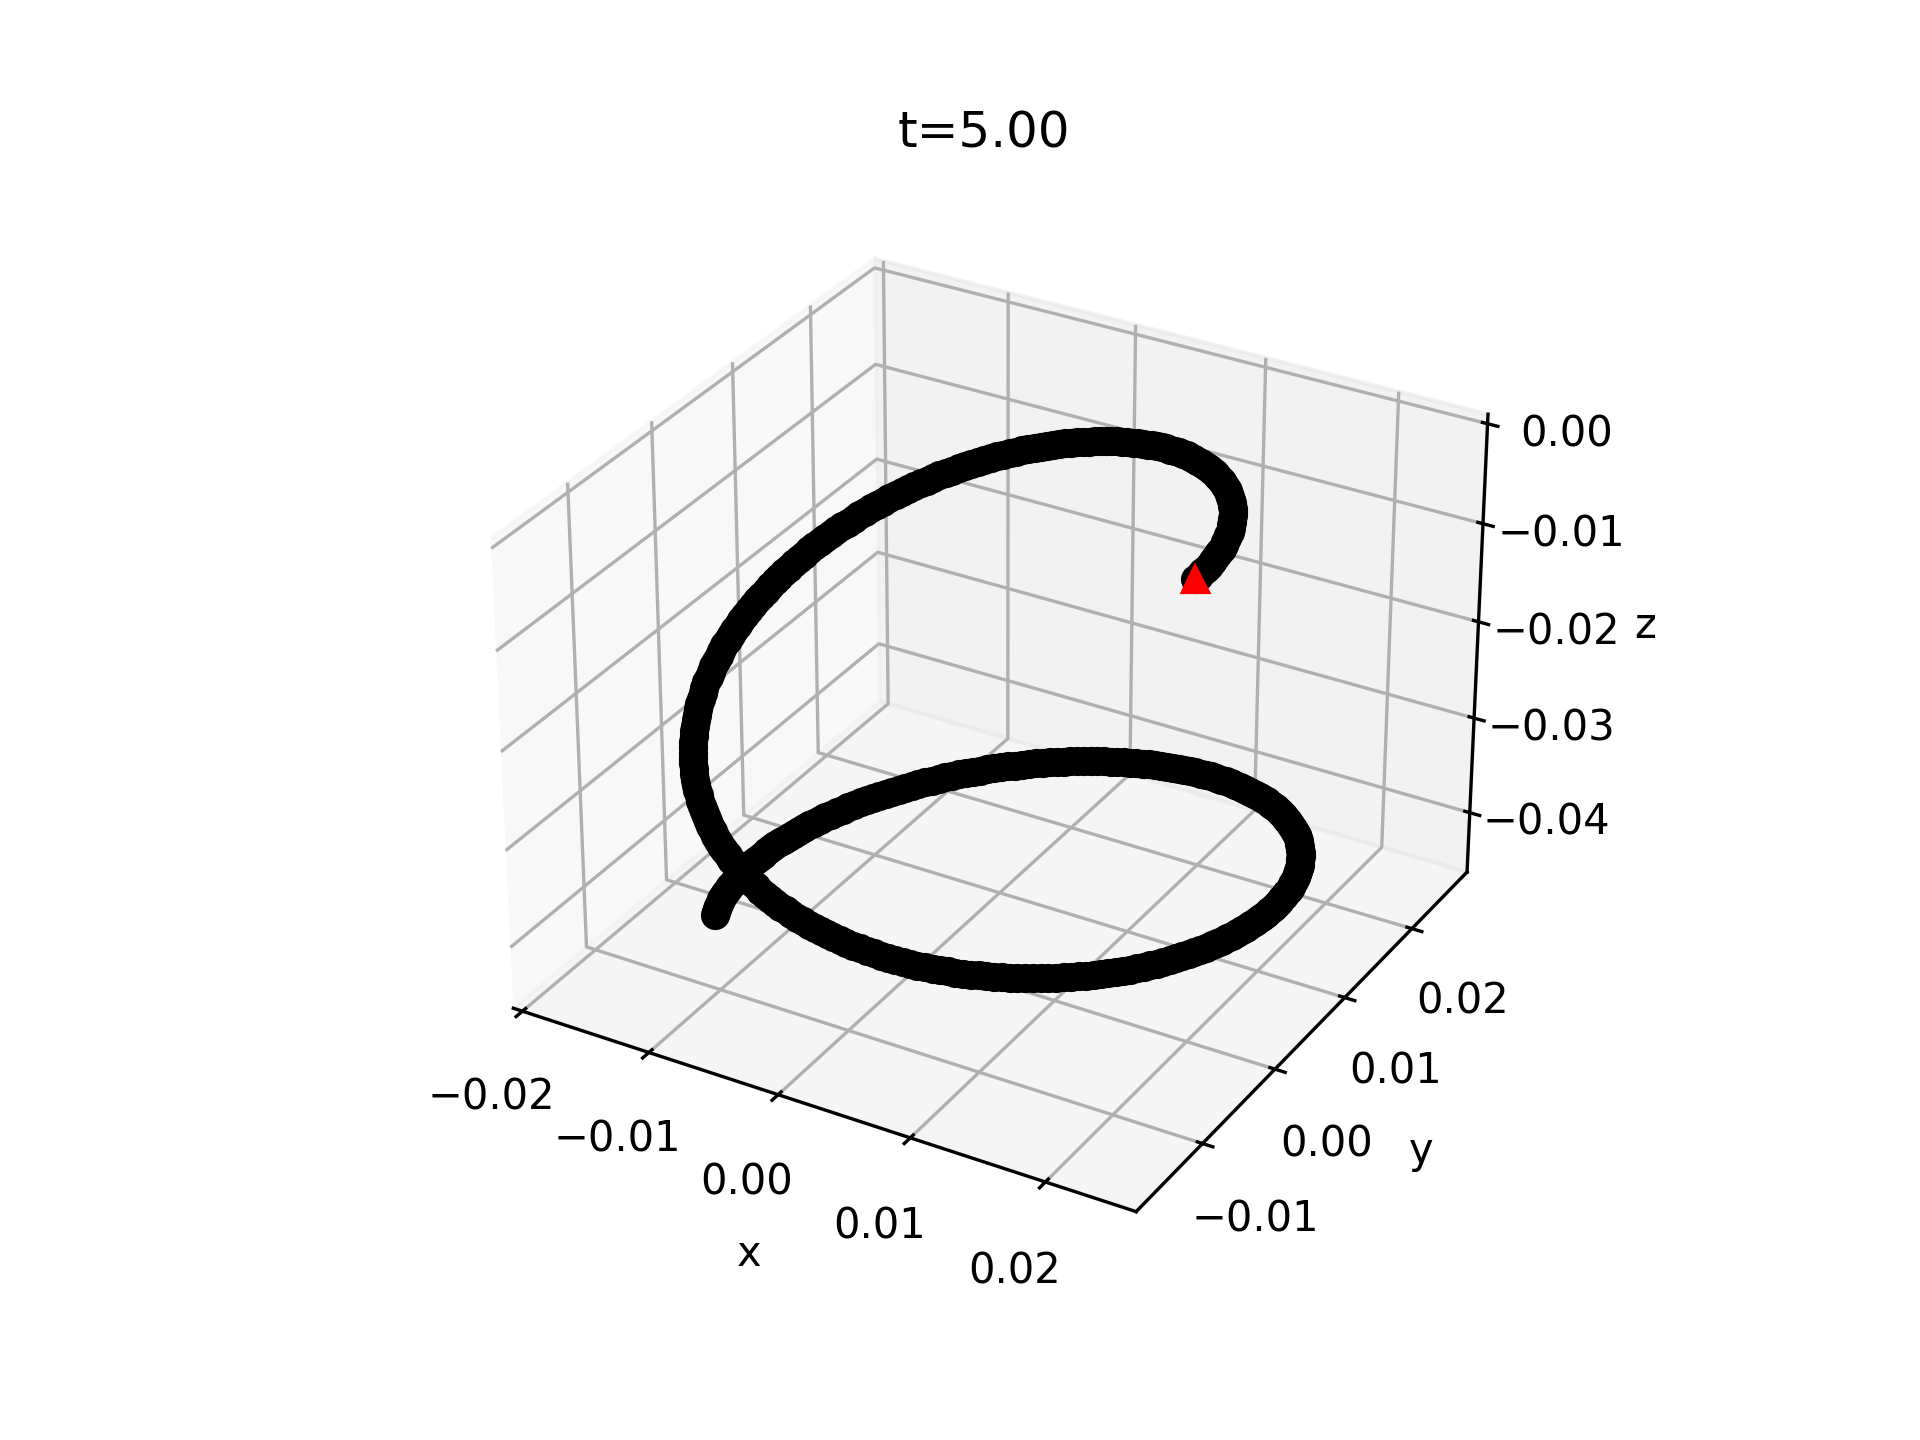
\includegraphics[width=0.8\linewidth]{../figures/n_400_dt_0-005_t=5s.png}
   \caption{The most accurate simulation, ending pose ($N=400$, $\Delta t = 0.005$s)}
   \label{fig:accurate_end}
\end{figure}

\begin{figure}[h!]
   \centering
   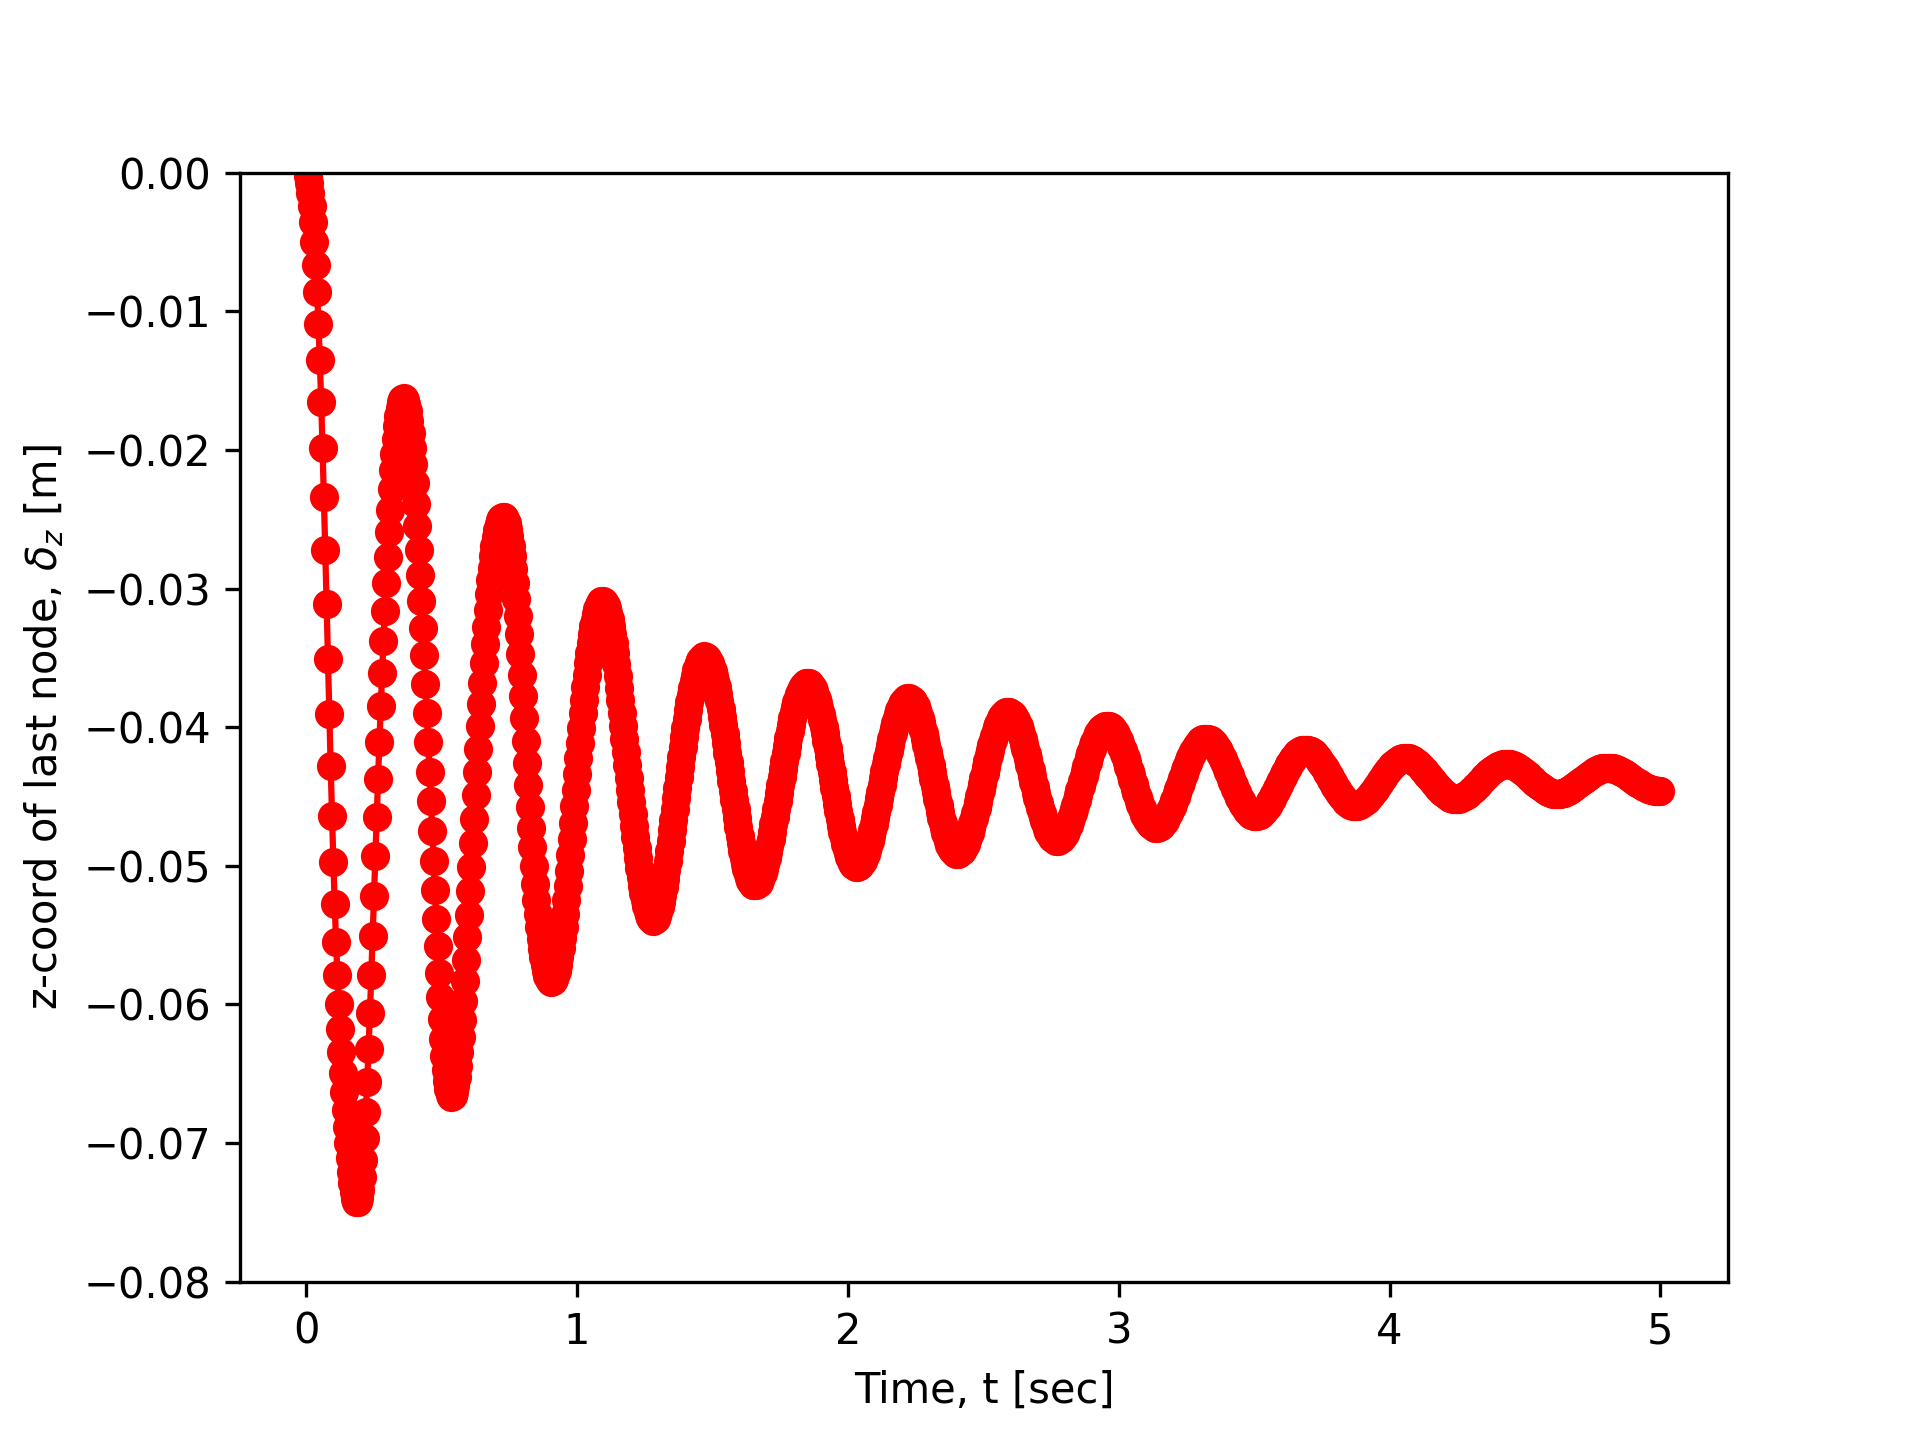
\includegraphics[width=0.8\linewidth]{../figures/n_400_dt_0-005_z_plot.png}
   \caption{The most accurate simulation, plot of z-coordinates for last node ($N=400$, $\Delta t = 0.005$s)}
   \label{fig:accurate_zplot}
\end{figure}

\subsection{Sensitivity Analysis}

Sensitivity analysis was performed to determine the requirements on the refinement of mesh for accurate results.
The mesh is constructed parametrically by defining the number of nodes $N$ and the time-step in the simulation $\Delta t$.

\begin{figure}[h!]
   \centering
   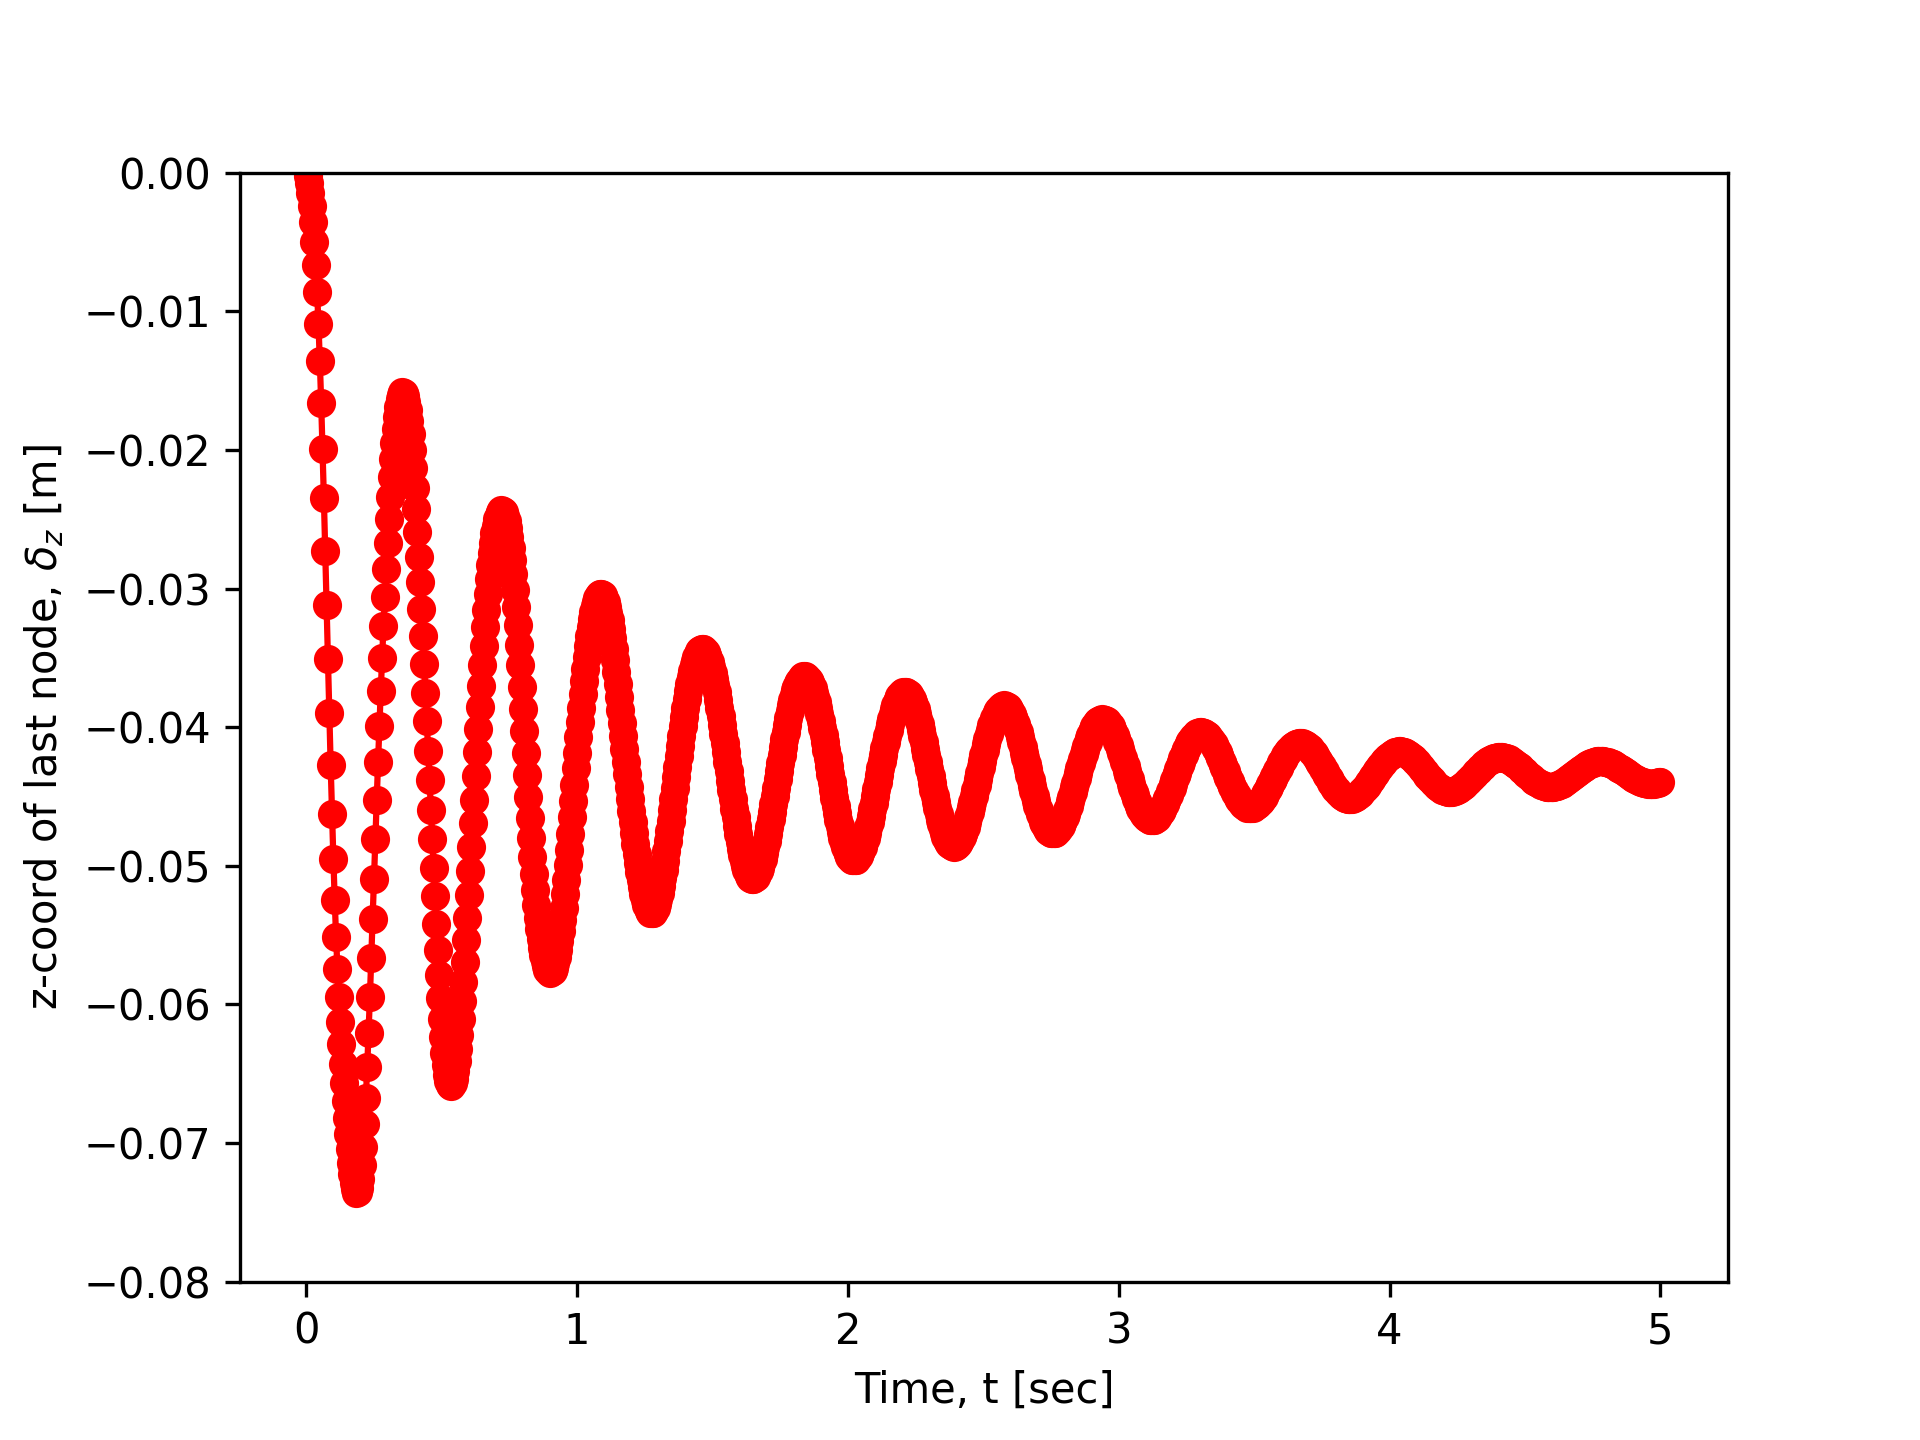
\includegraphics[width=0.8\linewidth]{../figures/n_100_dt_0-005_z_plot.png}
   \caption{Decreasing Number of Nodes ($k$), plot of z-coordinates for last node ($N=100$, $\Delta t = 0.005$s)}
   \label{fig:lessNodes_zplot}
\end{figure}

It is found that decreasing the number of nodes does not have significant impact on the results, as shown in Fig. \ref{fig:lessNodes_zplot}.
However, when we further increase the refinement of $\Delta t: 0.005 \rightarrow 0.001$, there is noticeable difference.
The damping effects on the system in converging to a steady state of $z \approx -0.04$ are less pronounced, and so steady state is not achieved in the $5s$ duration of this simulation.

\begin{figure}[h!]
   \centering
   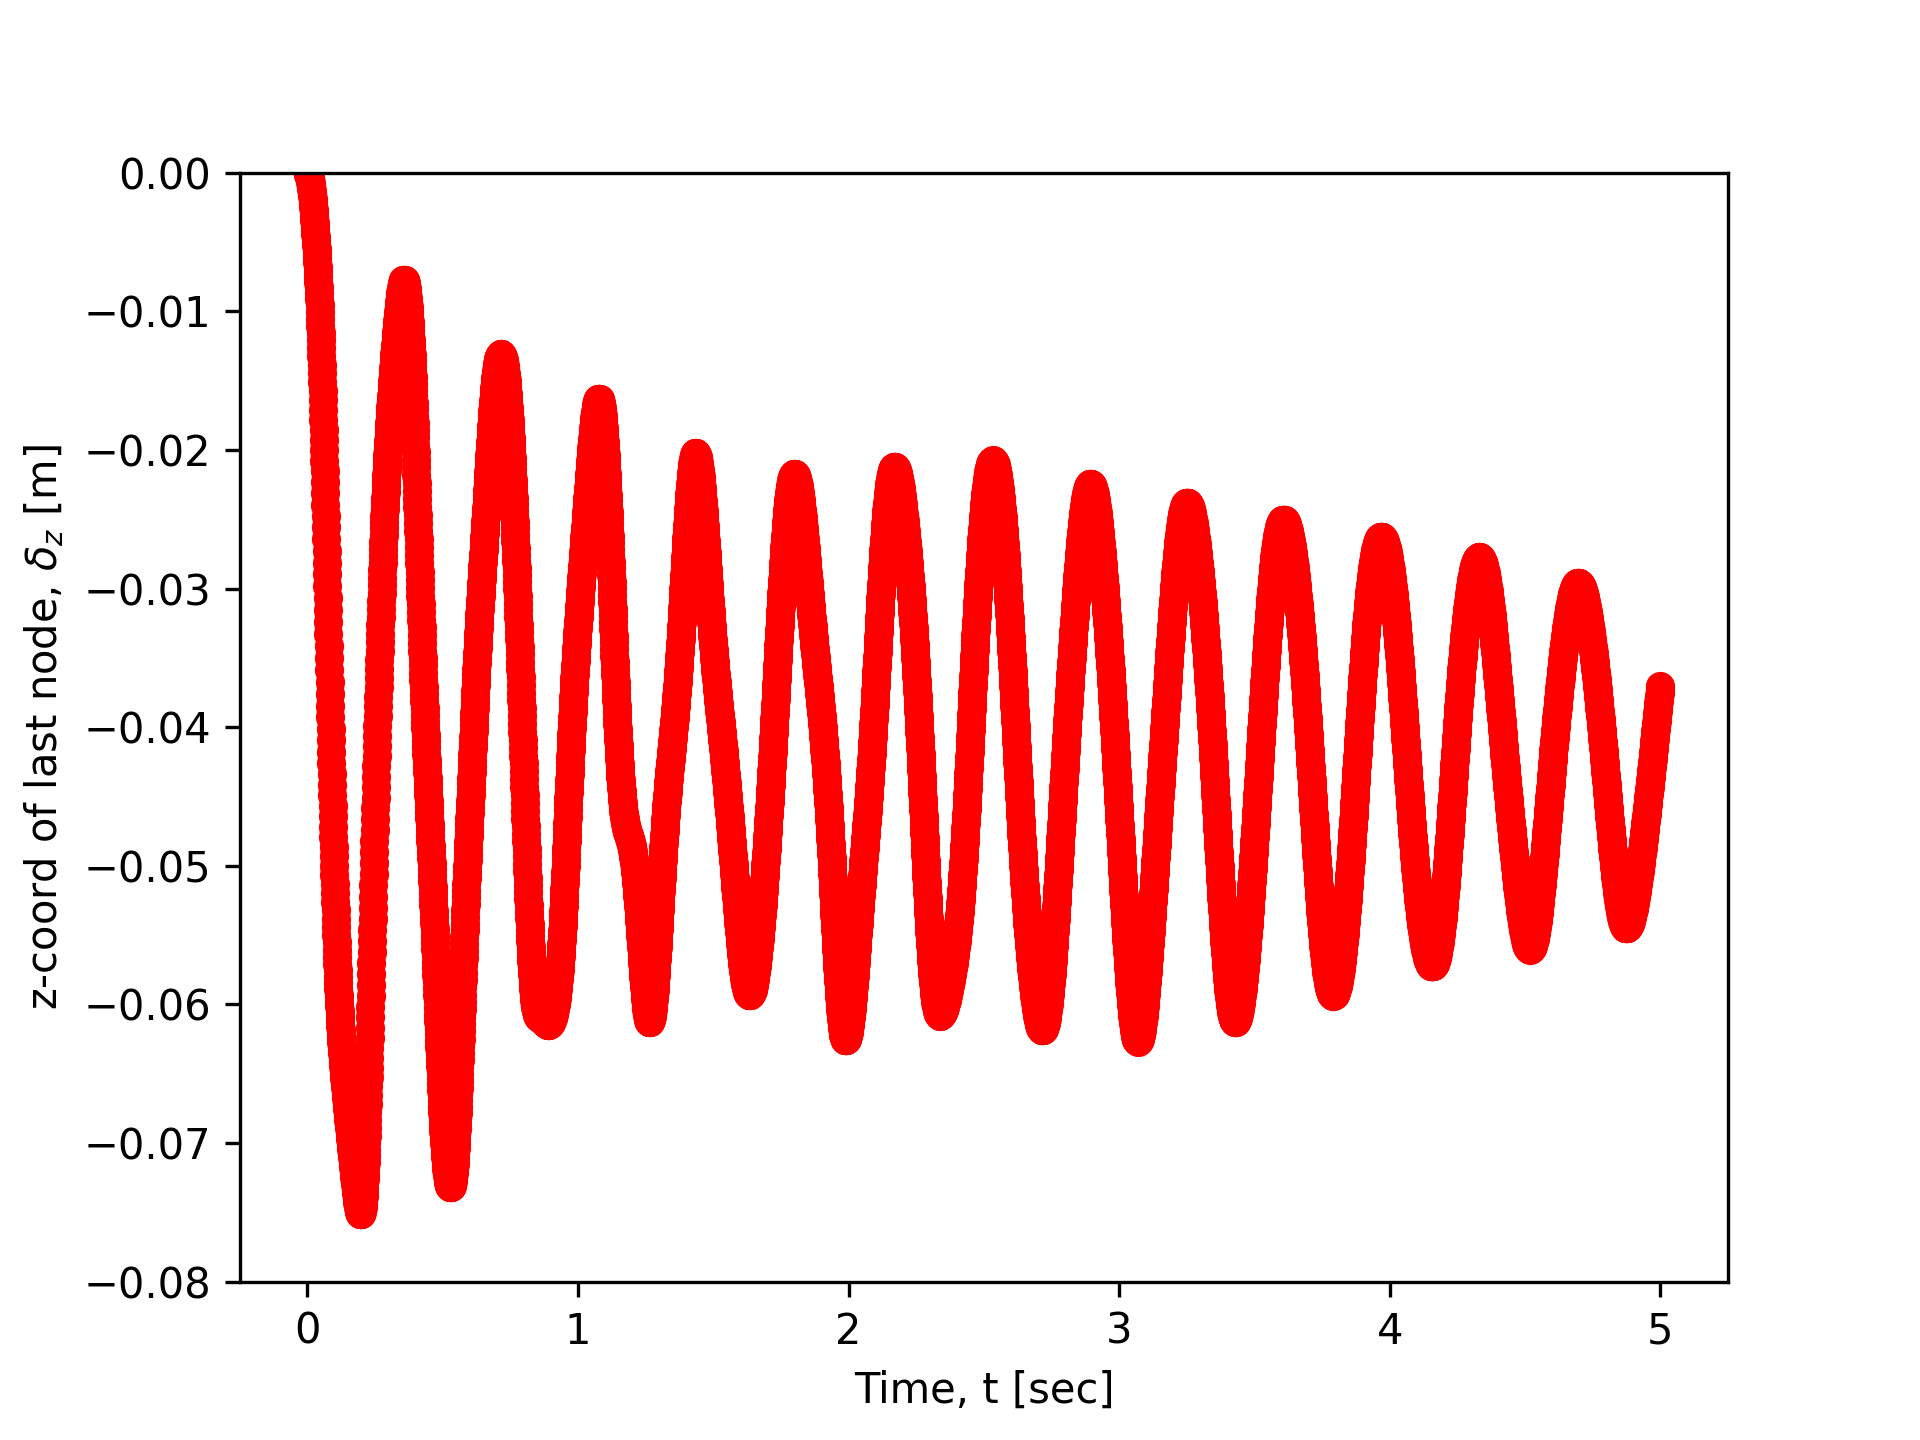
\includegraphics[width=0.8\linewidth]{../figures/n_50_dt_0-001_z_plot.png}
   \caption{Decreasing time steps for more refinement ($\Delta t$), plot of z-coordinates for last node ($N=50$, $\Delta t = 0.001$s)}
   \label{fig:lessDT_zplot}
\end{figure}

In either case of adjusting either $K$ or $\Delta t$, the trade off is computational time.
We note that refinement of $\Delta t$ is linearly correlated to the number of steps to be computed. 
In this case, each subsequent step of the simulation should take less iterations of Newton-Raphson to converge as the system approaches a steady state.
Still, as shown in Fig. \ref{fig:lessDT_zplot}, if there is no steady state achieved in the simulation, then the computational time for each step is approximately constant, and so the computational time for this simulation is linearly correlated with the refinement in $\Delta t$.

Alternatively, increasing the density of nodes $K$ has less noticeable effects on computational time, because the physics of nodes that are linked close together mean that there is less variance, and so the computational increase with a higher node density is not a linear correlation; it is intuitively logarithmic in nature.

\begin{figure}[h!]
   \centering
   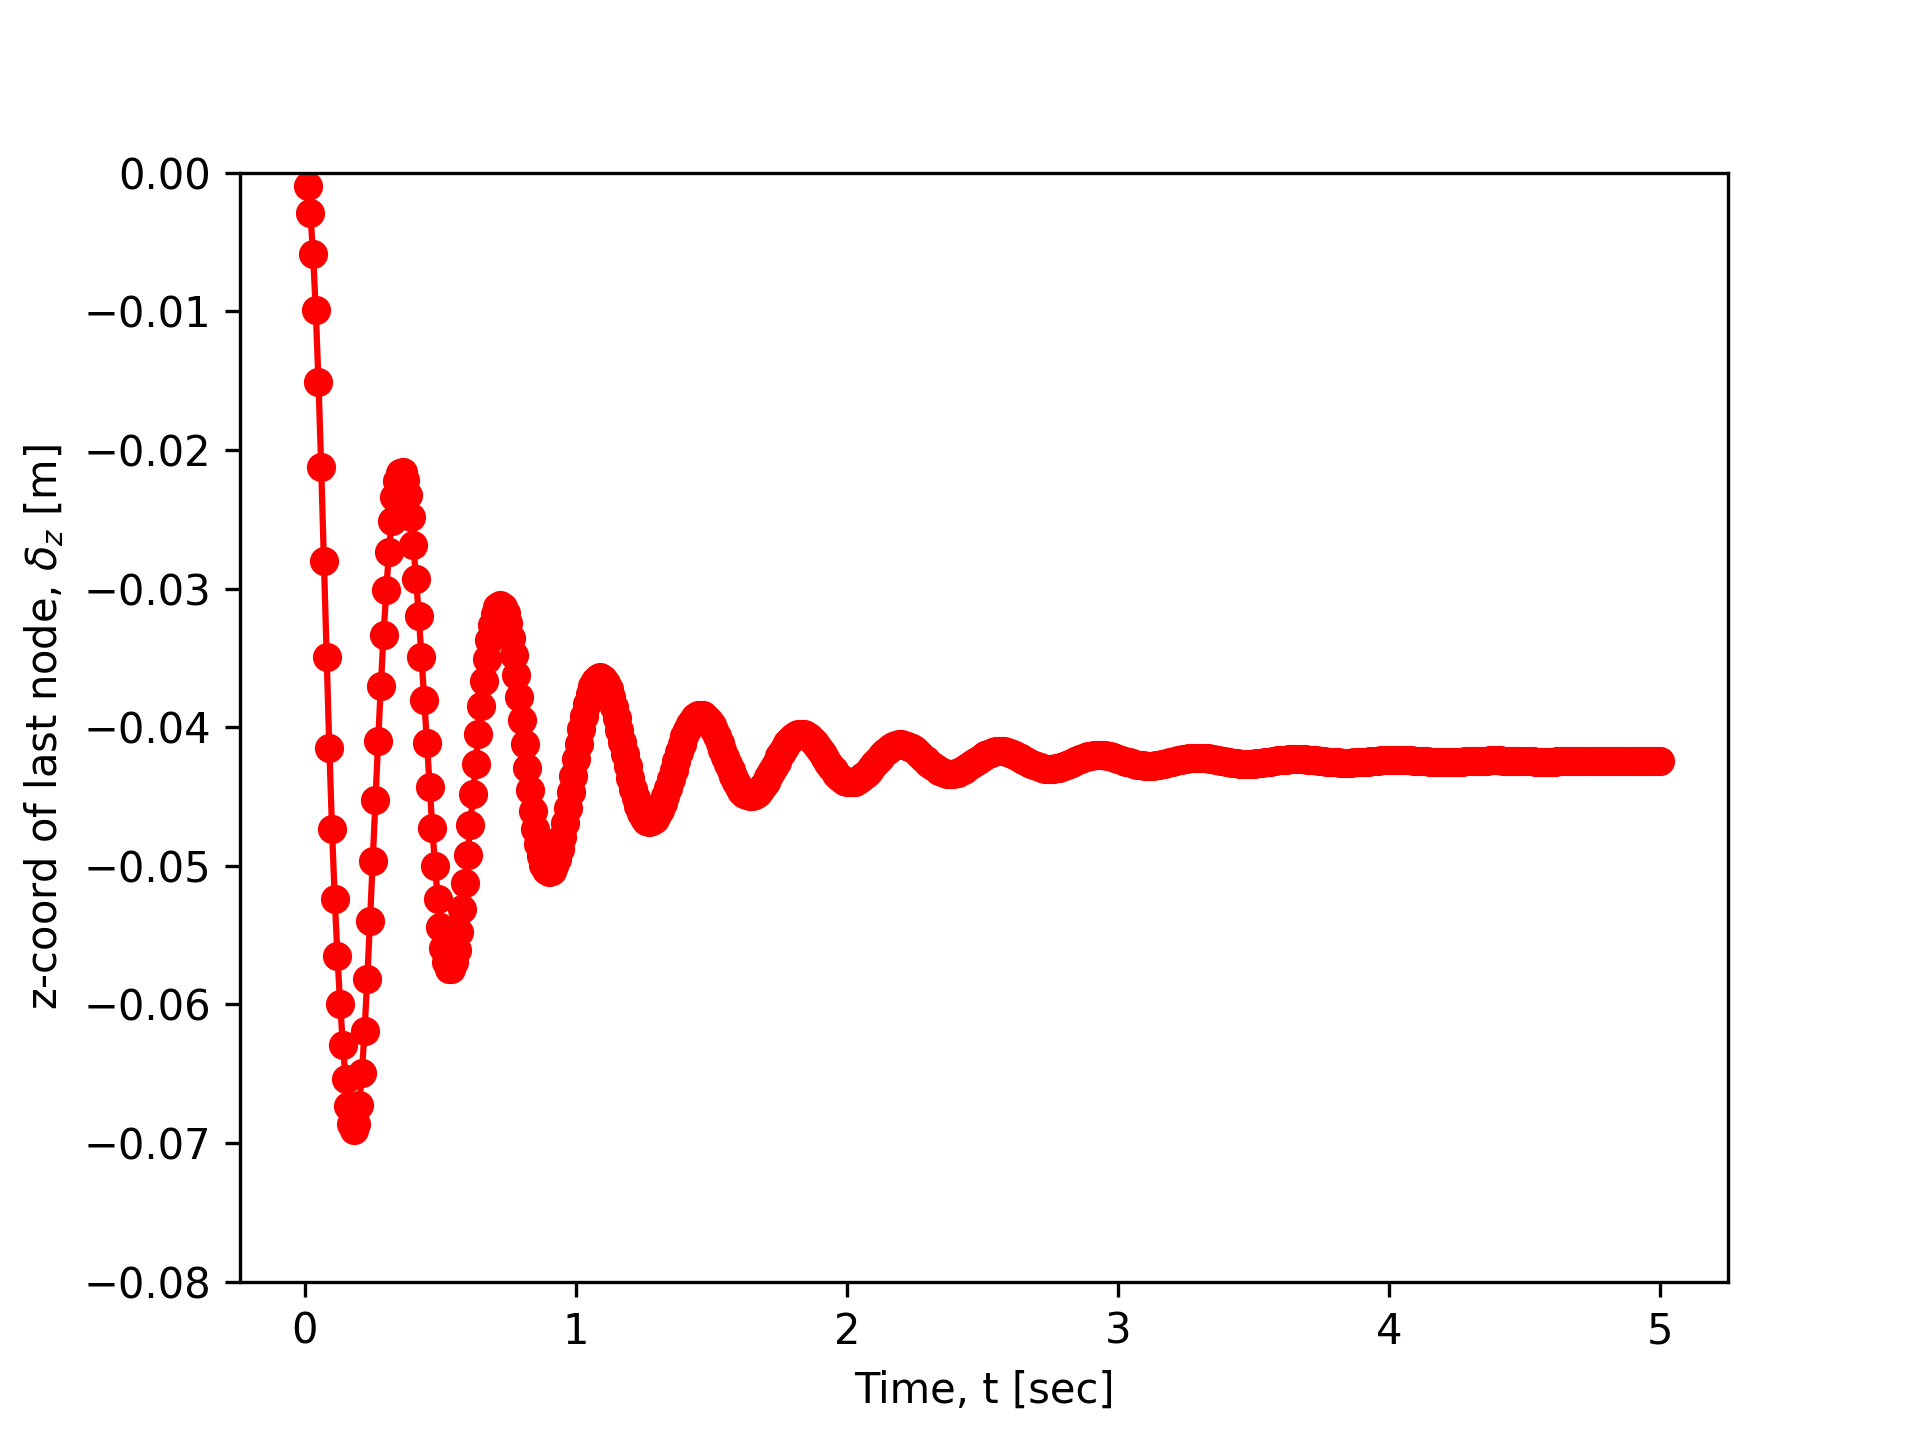
\includegraphics[width=0.8\linewidth]{../figures/n_50_dt_0-01_z_plot.png}
   \caption{Nominal plot of z-coordinates for last node ($N=50$, $\Delta t = 0.01$s)}
   \label{fig:nominal_zplot}
\end{figure}

For completness, we also furnish the nominal plot of z-coordinates in the last node for $N=50$, $\Delta t = 0.01$s, as is furnished in Chapter 7 of the text in this course.

%%%%%%%%%%%%%%%%%%%%%%%%%%%%%%%%%%%
\section*{ACKNOWLEDGMENT}

Material used in this report are taken from the course UCLA MAE 263F, Fall 2024.



%%%%%%%%%%%%%%%%%%%%%%%%%%%%%%%%%%%%%%%%%%%%%%%%%%%%%%%%%%%%%%%%%%%%%%%%%%%%%%%%

\begin{thebibliography}{99}

\bibitem{c1} M. Khalid Jawed, Singmin Lim, Discrete Simulation of Slender Structures, UCLA Fall 2024 MAE 263F

\end{thebibliography}


\end{document}
